\chapter{Methodology}

The sound containing the data in a text file is created with the DosSend program. It will be read back with DosRead to see how efficiently it can process the signal without altering the data it contains.

\section{DosSend and DosRead usage}

\subsection{Using DosSend to create a wav file}

\subsubsection{Compiling the Program}

Compile the Java code using a Java compiler

\begin{lstlisting}
javac DosSend.java StdDraw.java
\end{lstlisting}

\subsubsection{Run the Program}

Run DosSend with Java and send it your data written in a .txt file via standard input.

\begin{lstlisting}
java DosSend < textfile.txt
\end{lstlisting}

\subsubsection{Output}

The program will convert the input text into an audio signal and save it as \texttt{DosOok\_message.wav}. It will also print characteristics of the signal to the console and display a graphical representation of the signal waveform. It is a sinusoïdal wave modulated using OOK modulation.

\begin{figure}[!h]
	\begin{lstlisting}[style=console]
[oli@oli-arch src]$ java DosSend < helloWorld.txt
[ H e l l o   W o r l d   ! ]
[ 1 0 1 0 1 0 1 0 0 0 0 1 0 0 1 0 1 0 1 0 0 1 1 0 0 0 1 1 0 1 1 0 0 0 1 1 0 1 1 0 1 1 1 1 0 1 1 0 0 0 0 0 0 1 0 0 1 1 1 0 1 0 1 0 1 1 1 1 0 1 1 0 0 1 0 0 1 1 1 0 0 0 1 1 0 1 1 0 0 0 1 0 0 1 1 0 0 0 0 0 0 1 0 0 1 0 0 0 0 1 0 0 ]
Message : Hello World !
Nombre de symboles : 13
Nombre d'échantillons : 49392
Durée : 1.12 s
	\end{lstlisting}
	\caption{Console output for the text "Hello World !"}
\end{figure}

\begin{figure}[!h]
	\begin{center}
		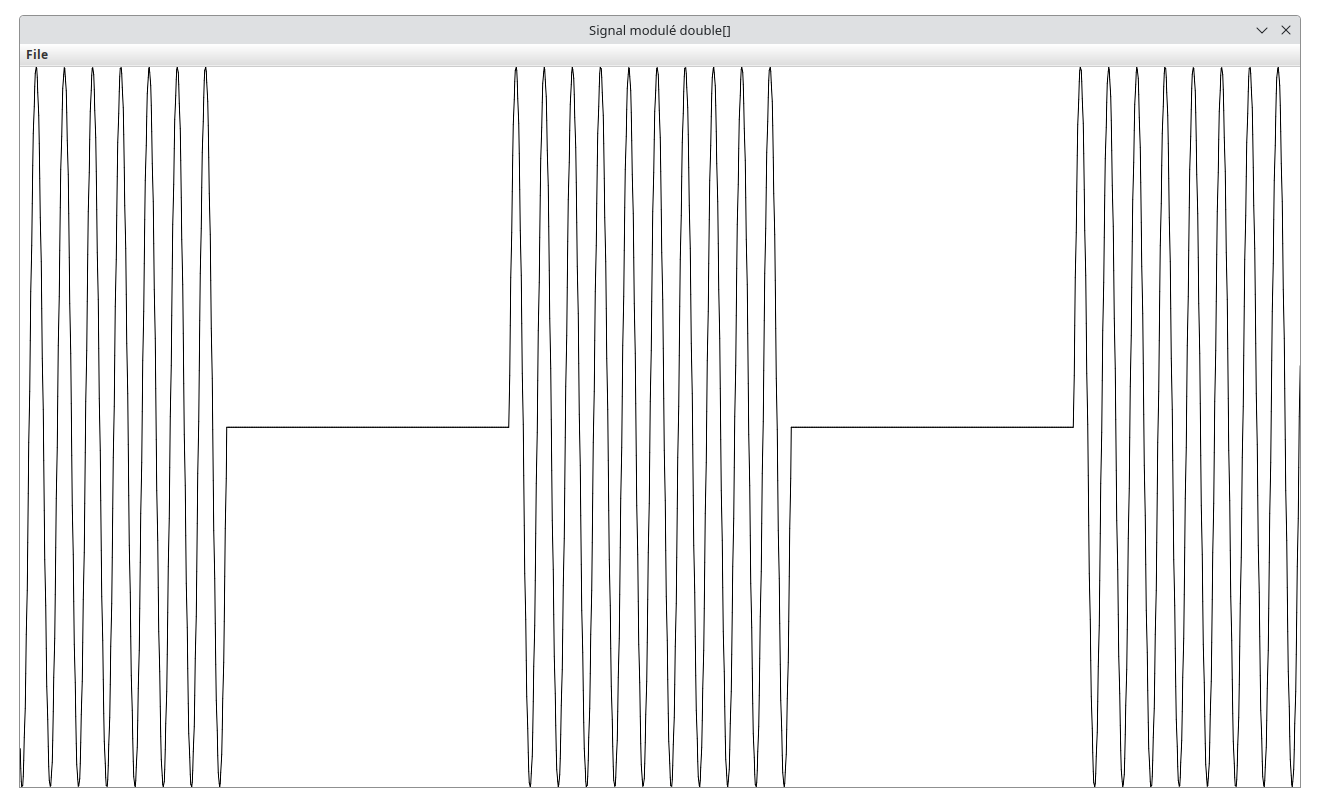
\includegraphics[width=15cm]{images/StdDraw1.png}
	\end{center}
	\caption{Signal output for the text "Hello World !" with start:300 stop:1000 mode:line}
\end{figure}

\subsection{Using DosRead}

\subsubsection{Compiling the Program}

Compile the Java code using a Java compiler

\begin{lstlisting}
javac DosSend.java StdDraw.java
\end{lstlisting}

\subsubsection{Run the Program}

Run DosRead with Java and add your sound file as a parameter.

\begin{lstlisting}
java DosRead sound.wav
\end{lstlisting}

\subsubsection{Output}

The program will read, process (through a low pass filter), and analyze audio data from the \texttt{WAV} file. It will then output information about the file and the text corresponding to the binary sequence to a terminal. It will show a graphical representations of the original signal and it's filtered counterpart.

\begin{figure}[!h]
	\begin{lstlisting}[style=console]
[oli@oli-arch src]$ java DosRead DosOok_message_sample.wav
Fichier audio: DosOok_message_sample.wav
Sample Rate: 44100 Hz
Bits per Sample: 16 bits
Data Size: 97660 bytes
Message décodé :    H e l l o   W o r l d   !
	\end{lstlisting}
	\caption{Console output for a wav file containing the text "Hello World !"}
\end{figure}

\begin{figure}[!h]
	\begin{center}
		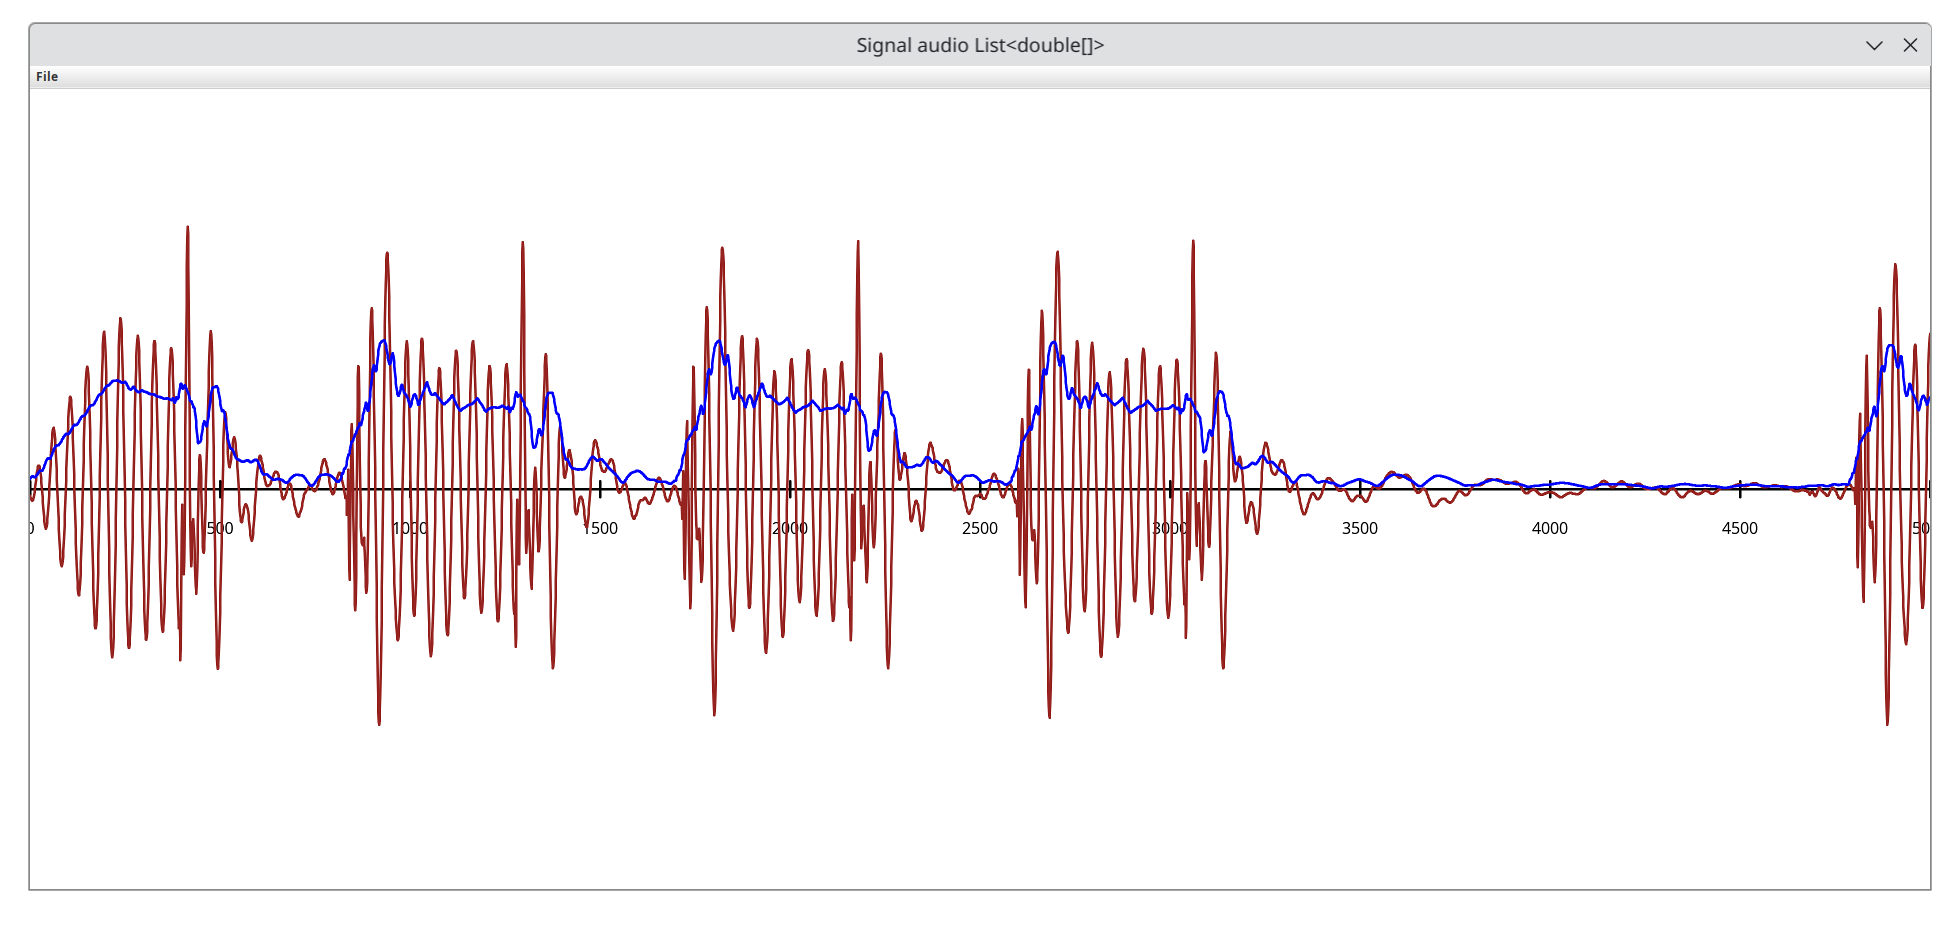
\includegraphics[width=15cm]{images/StdDraw2.png}
	\end{center}
	\caption{Signal output for the text "Hello World !". In red the signal before processing, in blue the same signal after processing}
\end{figure}

\newpage

\section{Explanation of the Low-Pass Filters}

\subsection{LPFilter1 : Moving Average Filter}

The moving average filter is a basic type of Low Pass FIR filter that is widely employed to smooth out a sequence of data points or a signal. It operates by averaging a set number, M, of input samples at once, and then outputs a single averaged data point. While this method is effective for signals that are relatively free from noise, its performance significantly deteriorates when dealing with noisy signals.

\subsection{LPFilter2 : Exponential Moving Average Filter}

The exponential moving average (EMA) filter is a type of discrete, low-pass, infinite-impulse response (IIR) filter. It prioritizes recent data by giving it more weight and discounting older data in an exponential manner. This behavior is similar to the discrete first-order low-pass RC filter. In contrast to a simple moving average (SMA) this ensures that the trend is maintained by still considering a significant portion of the reactive nature of recent data points. Compared to the SMA, this filter effectively suppresses noisy components, making it optimal for denoising signals in the time domain. It is a 1st order infinite impulse response (IIR) filter.

\section{Method to monitor the speed and accuracy of the filters}

\subsection{Monitoring the speed of the filters}

Each filter will process 3 files : A short one (two words), A medium one (one paragraph, 97 words), A long one (10 paragraphs, 939 words). Each of the wav files will have been created with DosSend.java and processed within DosRead.java. This will create ideals conditions for the filters as the noise will be minimal. For each files 3 settings with increased filtering power will be used and each of them must not alter DosRead decoding capability.

\subsection{Monitoring the accuracy of the filters}

Each filter will process 3 files with noise added to it : A clean one, A noisy one and A noisier one.

